\section{Experimenteller Teil}
Im ersten Teil der Auswertung verfolgen wir im Wesentlichen Ionen durch die Anlage.
Untersucht werden soll dabei eine vorbereitete BeO-Probe.
Im zweiten Teil betrachten wir aufgenommene Spektren und untersuchen eine unbekannte Probe.

\subsection{Auf dem Weg zum Beschleuniger}
Nach der Produktion der negativen Ionen durch sputtern werden diese direkt mit insgesamt \SI{29}{\kilo\electronvolt} beschleunigt.
Sie durchlaufen dann eine elektrostatischen Analysierer und einen ersten Ablenkmagneten.
Das Ziel hier ist eine Ionenmasse vorzuselektieren.
Da wir BeO untersuchen sind mögliche gesuchte Ionen $^{9}\text{Be}^{16}\text{O}^{-}$ (stabiles Beryllium-Iosotop) und $^{10}\text{Be}^{16}\text{O}^{-}$ (radioaktives Beryllium-Iostop mit einer Halbwertszeit von \num{1.51e6} Jahren).
Wir kennen die kinetische Energie $E_{\text{kin}}$, den Ladungszustand $q_{\text{ion}}$, die Masse der Ionen $m_{\text{ion}}$ und den Krümmungsradius der weiterführenden Trajektorie $\rho$.
Daher kann man durch geeignete Wahl der Stärke des Magnetfeldes die Ionenmasse auswählen:
\begin{gather}
    B \rho = \frac{p_{\text{ion}}}{q_{\text{ion}}} = \frac{\sqrt{2m_{\text{ion}}E_{\text{kin}}}}{q_{\text{ion}}}
    \label{Auswertung_eq_Magnet}
\end{gather}
Ionen mit einer anderen Masse oder anderem Ladungszustand haben im Magneten eine anders gekrümmte Trajektorie und gelangen daher nicht durch die Eintrittsöffnung zum Beschleuniger.
(Tatsächlich lässt sich wie in Gleichung \ref{Auswertung_eq_Magnet} zu sehen nur nach $\frac{\sqrt{m_{\text{ion}}}}{q_{\text{ion}}}$ selektieren.
Ionen mit vierfacher Masse und doppelter Ladung würden also auch weiterkommen. Derart schwere Teilchen sind jedoch fast gar nicht in der Probe vorhanden.)
Nicht unterscheiden lässt sich jedoch zwischen Molekularen isobaren, so zum Beispiel zwischen $^{10}\text{Be}^{16}\text{O}^{-}$ und $^{9}\text{Be}^{17}\text{O}^{-}$ (wobei $^{17}\text{O}$ in der Natur sehr selten vorkommt) oder $^{10}\text{Be}^{16}\text{O}^{-}$ und $^{10}\text{B}^{16}\text{O}^{-}$ ($^{10}\text{B}$ entsteht beim Beta-Zerfall von $^{10}\text{Be}$).
Für $\rho$ war ein Wert von \SI{0.4}{\metre} gegeben.
Damit ergeben sich für einfach negativ geladene Ionen folgende benötigte Magnetfeldstärken:
\begin{table}[h]
  \centering
  \begin{tabular}{|c|c|}
    \hline
    Ion & Magnetfeldstärke \\
    \hline
    $^{9}\text{Be}^{16}\text{O}^{-}$ & \SI{-0.306}{\tesla} \\
    \hline
    $^{10}\text{Be}^{16}\text{O}^{-}$ & \SI{-0.313}{\tesla} \\
    \hline
  \end{tabular}
  \caption{Benötigte Magnetfeldstärken im ersten Ablenkmagneten für Ionen vor dem Beschleuniger}
  \label{Auswertung_tab_Ionenenergien_vor_Besch}
\end{table}
Um diese Magnetfelder anzulegen ist eine Kalibrierung des Magneten erforderlich, die jedoch in diesem Versuch nicht durchgeführt wurde.
Unsicherheiten der Beschleunigungsspannungen und des Spulenradius werden hier nicht betrachtet, da sie gegenüber der variablen Hysterese des Magneten kaum einen Einfluss auf die Unsicherheit der Ablenkung haben.
Diese wiederrum wäre ebenfalls am besten experimentell (z.B. mittels Hall-Sonde) zu bestimmen.

\subsection{Teilchenenergien nach dem Beschleuniger}
Die Vorselektierten Ionen werden im ersten Teil des Beschleunigers mit der angelegten Spannung beschleunigt.
In der Mitte treffen sie auf Argon an welchem sie sich umladen und die Moleküle aufbrechen.
(Das Aufbrechen der Moleküle ist kein Problem, da chemische Bindungsenergien typischerweise im \si{\electronvolt}-Bereich liegen, die Ionen bis dahin aber schon mehrere \si{\mega\electronvolt} an kinetischer Energie haben.)
Die entstandenen Ionen werden dann mit ihrer positiven Ladung noch ein weiteres Mal mit der angelegten Spannung beschleunigt.
Daher ergibt sich ihre Energie nach dem Beschleuniger zu:
\begin{gather}
    E_{\text{tot}} = e \cdot (U_{\text{Ionenquelle}} + U_{\text{Beschleuniger}}) \cdot \frac{m_{\text{Ion}^{+}}}{m_{\text{Molekül}^{-}}} + U_{\text{Beschleuniger}} \cdot q_{\text{Ion}^{+}}
\end{gather}
Wobei im erste Summand der Term $\frac{m_{\text{Ion}^{+}}}{m_{\text{Molekül}^{-}}}$ benutzt wird um die anteilige kinetische Energie des entstandenen Ions bis zum Argongas zu beschreiben.
Der zweite Summand beschreibt die Beschleunigung nach dem Argongas.

In unserem Versuch betrug die Spannung des Beschleunigers \SI{5.2479e6}{\volt}.
Damit ergeben sich für entstandene Ionen eine Energie nach dem Beschleuniger von:
\begin{center}
  \begin{tabular}{|c|c|}
    \hline
    Ion & Energie \\
    \hline
    $^{9}\text{Be}^{1+}$ & \SI{7.1}{\mega\electronvolt} \\
    $^{9}\text{Be}^{2+}$ & \SI{12.3}{\mega\electronvolt} \\
    $^{9}\text{Be}^{3+}$ & \SI{17.6}{\mega\electronvolt} \\
    $^{9}\text{Be}^{4+}$ & \SI{22.8}{\mega\electronvolt} \\
    \hline
    $^{10}\text{Be}^{1+}$ & \SI{7.3}{\mega\electronvolt} \\
    $^{10}\text{Be}^{2+}$ & \SI{12.5}{\mega\electronvolt} \\
    $^{10}\text{Be}^{3+}$ & \SI{17.8}{\mega\electronvolt} \\
    $^{10}\text{Be}^{4+}$ & \SI{23.0}{\mega\electronvolt} \\
    \hline
    $^{16}\text{O}^{1+}$ & \SI{8.5}{\mega\electronvolt} \\
    $^{16}\text{O}^{2+}$ & \SI{13.7}{\mega\electronvolt} \\
    $^{16}\text{O}^{3+}$ & \SI{19.0}{\mega\electronvolt} \\
    $^{16}\text{O}^{4+}$ & \SI{24.2}{\mega\electronvolt} \\
    \hline
  \end{tabular}
  \captionof{table}{Ionenenergien nach dem Beschleuniger für ausgewählte Ionen}
  \label{Auswertung_tab_Ionenenergien_nach_Besch}
\end{center}

\subsection{Faraday-Cups}
Nachdem wir nun Ionen mit hoher Geschwindigkeit nach dem Beschleuniger haben können wir versuchen häufig auftretende Nuklide nachzuweisen.
Aufgrund der hohen Anteile dieser Nuklide im Telichenstrahl entsteht durch sie ein nennenswerter Ladungsstrom der mit sogenannten Faraday-Cups gemessen werden kann.
Um einzelne Ionsorten detektieren zu können ist nach dem Beschleuniger ein \ang{90} Ablenkmagnet angebracht, der funktioniert wie der auf der Niederenergieseite.
Auch hier ist die Kalibrierung des Magneten uns nicht bekannt.
Im Faraday-Cup werden dann die auftreffenden Ströme gemessen, die bei einem bestimmten Strom durch die Spule durch die abgelenkten Ionen entsteht.
Zunächst wollen wir sehen ob sich die Nuklide unserer BeO-Probe nachweisen lassen.
Dafür wurde in Abb. \ref{Auswertung_Bild_Faraday_Cup_BeO_HE} die gemessenen Ionenströme über dem Strom durch den Ablenkmagneten aufgetragen.
\begin{figure}[ht]
	\centering
    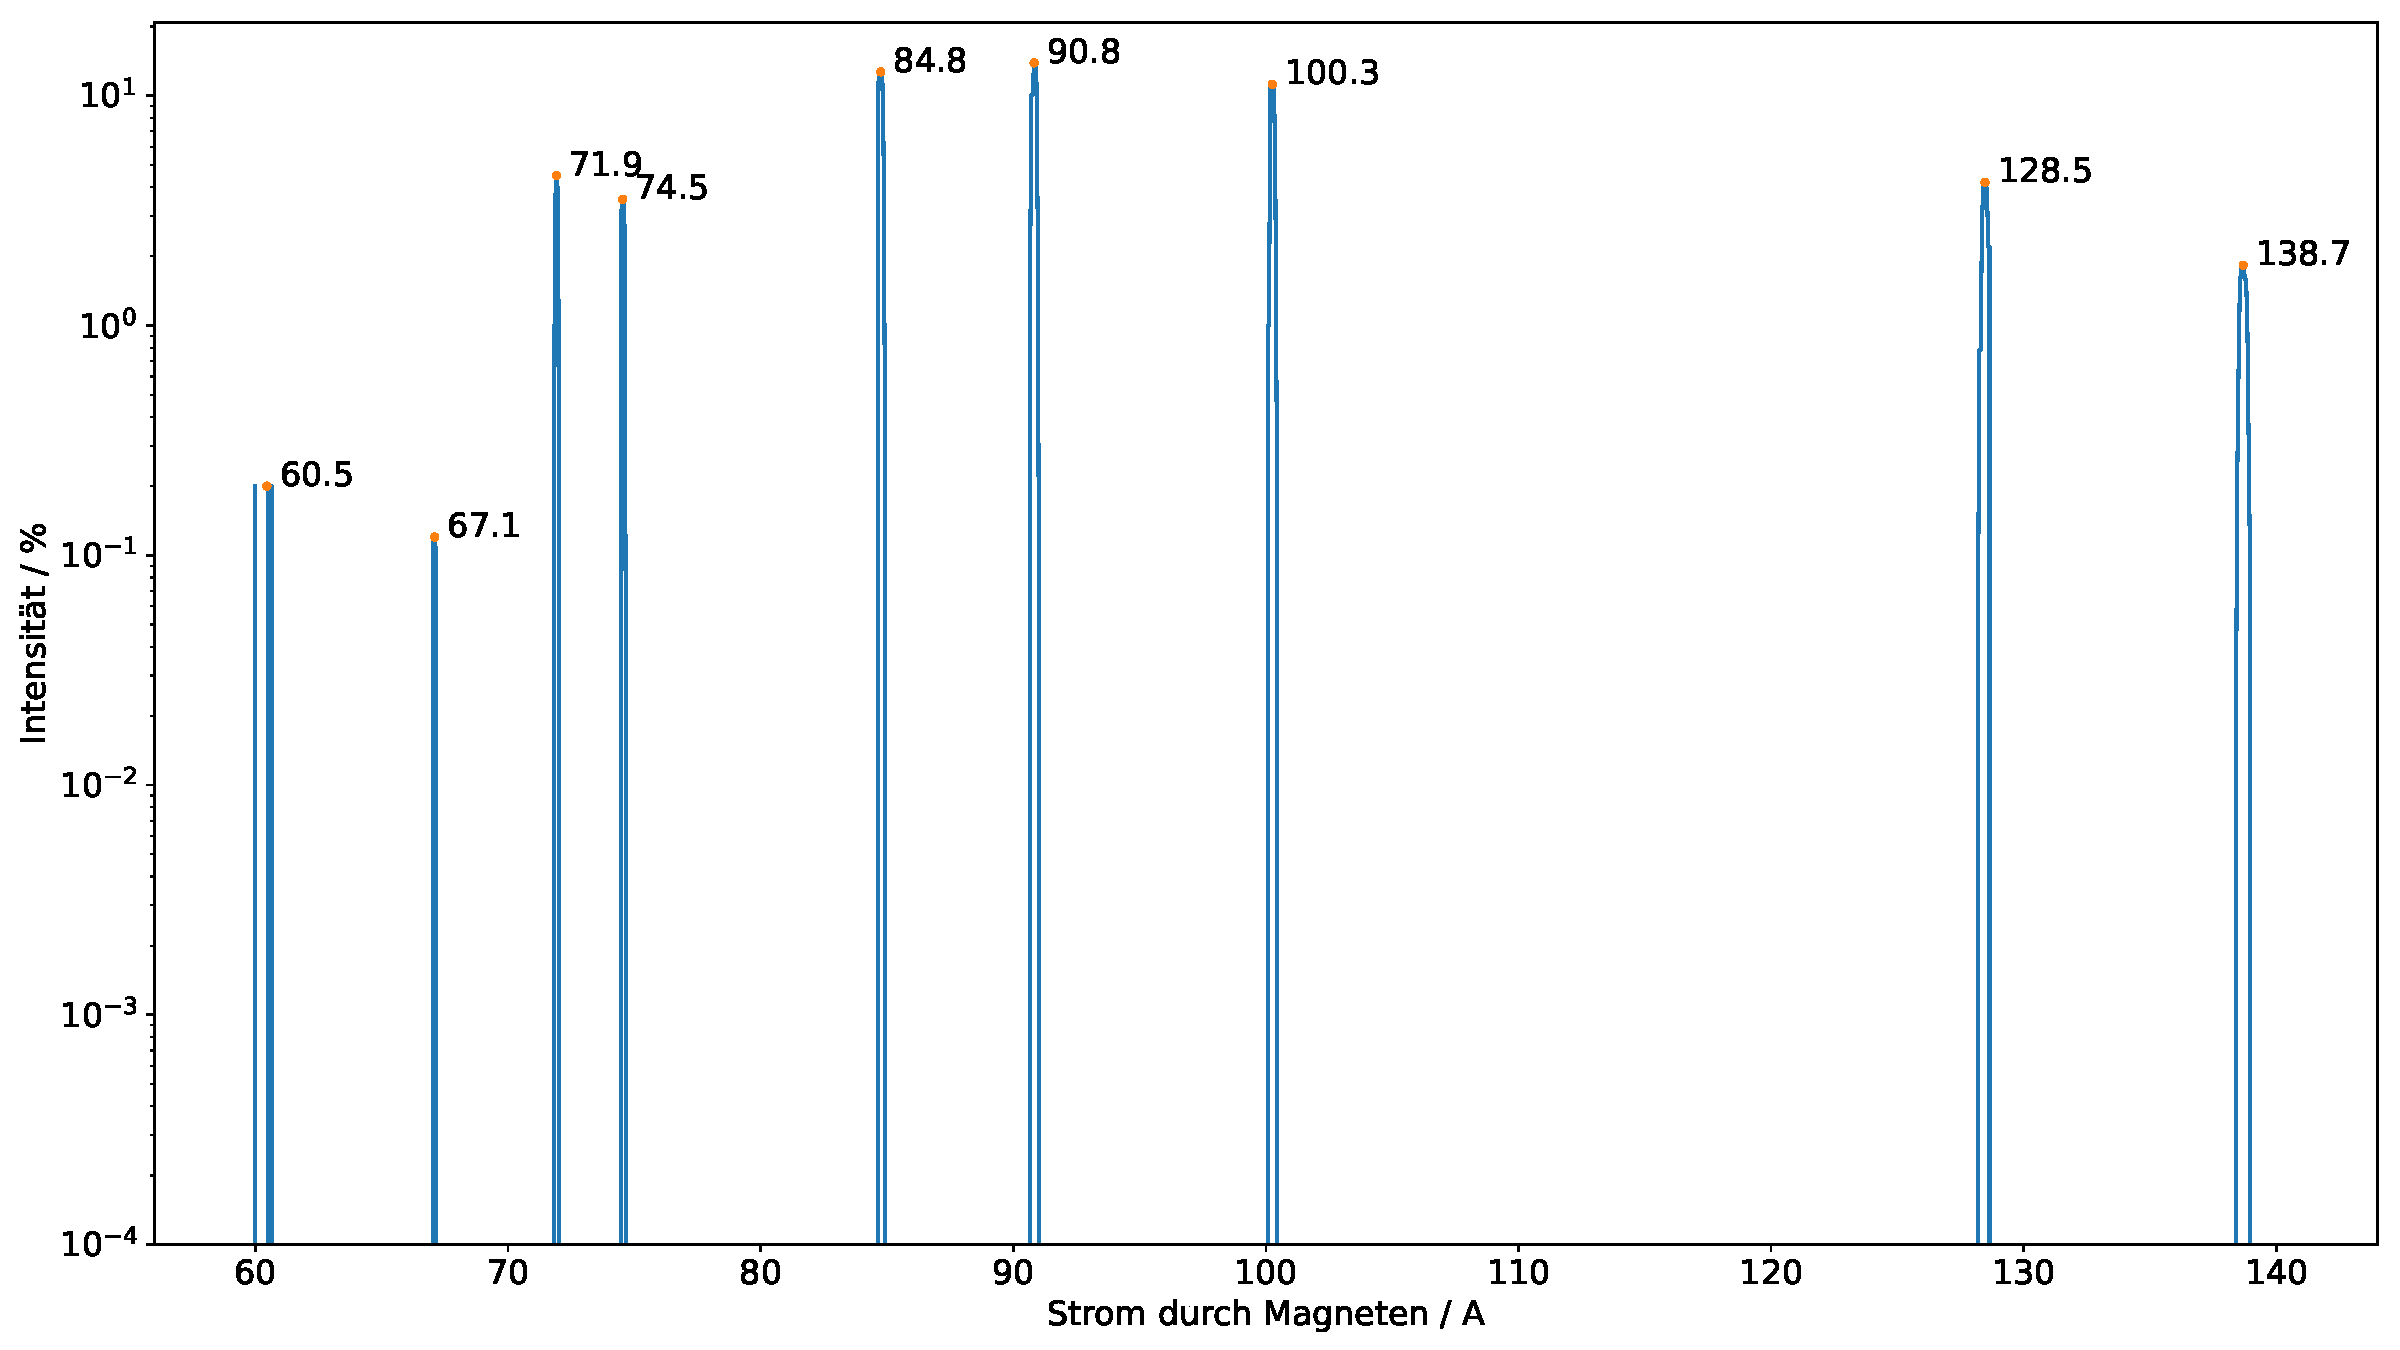
\includegraphics[width=0.85\textwidth]{Pictures/Faraday_Cup_BeO_HE.pdf}
	\caption{Strom gemessen im Faraday-Cup bei variieren des Magnetfeldes auf der Hochenergieseite für BeO-Probe. Die gemittelten x-Werte der Peaks sind eingezeichnet. Die Peaks wurden durch Vergleich mit umliegenden Werten gefunden. Die genaue Position wurde dann ermittelt indem die umliegenden Werte mit ihren Intensitäten als Wichtung gemittelt wurden.}
	\label{Auswertung_Bild_Faraday_Cup_BeO_HE}
\end{figure}
Wäre die Kalibrierung des Magneten bekannt könnte man mithilfe von Formel \ref{Auswertung_eq_Magnet} einfach auf mögliche Ionenspezies bei jedem Peak schließen.
Da dies leider nicht der Fall ist muss man die Peaks untereinander vergleichen.
Mithilfe von Formel \ref{Auswertung_eq_Magnet} wird sofort klar, dass das variieren des Magnetfeldes die Teilchen nur proportional zu $\frac{\sqrt{m_{\text{ion}}}}{q_{\text{ion}}}$ sortieren kann.
Daher kann der relative Abstand der Peaks entlang der x-Achse Aufschluss über die Ionenspezies geben.
Dafür ist es jedoch notwendig zu wissen, welche Ionen man im Ionenstrahl möglicherweise erwartet.
Für die BeO-Probe wurden folgende Ionen für möglich erachtet:
\begin{center}
  \begin{tabular}{|c|c|c|c|}
    \hline
    Element & Masse $/\ \si{\atomicmassunit}$ & Ladungszustand $/\ e$ & $\frac{\sqrt{m_{\text{ion}}}}{q_{\text{ion}}}$\\
    \hline
    \multirow{8}*{Be}    & \multirow{4}*{$9$}  & $1+$                & \num{3}             \\
                         &                     & $2+$                & \num{1.5}           \\
                         &                     & $3+$                & \num{1}             \\
                         &                     & $4+$                & \num{0.75}          \\
    \cline{2-4}
                         & \multirow{4}*{$10$} & $1+$                & \num{3.16}          \\
                         &                     & $2+$                & \num{1.58}          \\
                         &                     & $3+$                & \num{1.05}          \\
                         &                     & $4+$                & \num{0.79}          \\
    \hline
    \multirow{4}*{O}     & \multirow{4}*{$16$} & $1+$                & \num{4}             \\
                         &                     & $2+$                & \num{2}             \\
                         &                     & $3+$                & \num{1.33}          \\
                         &                     & $4+$                & \num{1}             \\
    \hline
    \multirow{4}*{Al}    & \multirow{4}*{$26$} & $1+$                & \num{5.10}          \\
                         &                     & $2+$                & \num{2.55}          \\
                         &                     & $3+$                & \num{1.70}          \\
                         &                     & $4+$                & \num{1.27}          \\
    \hline
  \end{tabular}
  \captionof{table}{Mögliche Ionen auf Hochenergieseite für BeO-Probe.}
  \label{Auswertung_tab_moegl_ionen}
\end{center}
Dabei ist zu beachten das $^{10}\text{B}$ nicht von $^{10}\text{Be}$ unterschieden werden kann, und es daher auch keinen Sinn macht es mit aufzunehmen.
Isobare können erst im weiteren Verlauf getrennt werden.
Aluminium wurde aufgenommen, da es eine häufige Unreinheit in natürlich vorkommendem BeO ist, die ebenfalls zur Altersbestimmung genutzt werden kann.
Außerdem ist $^{26}\text{Al}$ in der Vorselektion nicht vom molekularen Isobar $^{10}\text{Be}^{16}\text{O}$ zu unterscheiden.
Man kann nun versuchen Permutationen dieser Ionen den Peaks zuzuordnen.
Davon gibt es $\frac{n!}{(n-r)!}$ wobei $n$ die Anzahl der möglichen Ionenspezies und $r$ die Anzahl der Peaks sind.
Das sind für $16$ Ionenspezies und $9$ Peaks über $4$ Milliarden.
Es genügt aber natürlich nur Permutationen zuzulassen, bei denen die Ionen nach steigendem $\frac{\sqrt{m_{\text{ion}}}}{q_{\text{ion}}}$ sortiert steigenden Strömen durch den Magneten zugeordnet werden.
Damit reduziert sich die Anzahl der Permutationen auf $\frac{n!}{r! \cdot (n-r)!}$.
Das sind für $16$ Ionenspezies und $9$ Peaks nur noch $11440$, also eine mit einem Computer in sinnvoller Zeit überprüfbare Anzahl.
Mithilfe geeigneter Normen (siehe Appendix \ref{Appendix_Normen}) lassen sich dann die Permutationen finden, die die Peaks am besten beschreiben.
Damit erhält man folgende Permutation als best-passende:
\begin{center}
  \begin{tabular}{|c|c|c|}
    \hline
    Peak $/\ \si{\ampere}$ & Peak-Intensität $/\ \%$ & Ion \\
    \hline
    \num{60.5} & \num{0.2} & $^{10}\text{Be}^{4+}$ \\
    \hline
    \num{67.1} & \num{0.1} & $^{16}\text{O}^{4+}$ \\
    \hline
    \num{71.9} & \num{4.5} & $^{9}\text{Be}^{3+}$ \\
    \hline
    \num{74.5} & \num{3.5} & $^{10}\text{Be}^{3+}$ \\
    \hline
    \num{84.8} & \num{12.7} & $^{26}\text{Al}^{4+}$ \\
    \hline
    \num{90.8} & \num{13.9} & $^{16}\text{O}^{3+}$ \\
    \hline
    \num{100.3} & \num{11.2} & $^{9}\text{Be}^{2+}$ \\
    \hline
    \num{128.5} & \num{4.2} & $^{26}\text{Al}^{3+}$ \\
    \hline
    \num{138.7} & \num{1.8} & $^{16}\text{O}^{2+}$ \\
    \hline
  \end{tabular}
  \captionof{table}{Zuordnung der Teilchenspezies zu den Peaks im Faraday-Cup bei variieren des Magnetfeldes auf der Hochenergieseite für BeO-Probe. Die Abweichung der Verhältnisse für gemessene / erwartete Peakpositionen mit euklidischer Norm ist \num{0.32} (Wurzel des Residuums bei Methode der kleinsten Fehlerquadrate)}
  \label{Auswertung_tab_Teilchenspezies_BeO_HE}
\end{center}
Die Intensitäten der Peaks wurden bisher noch gar nicht beachtet.
